\documentclass[10.5pt]{article}
\usepackage{xeCJK}%preamble part
\usepackage{graphicx}
\usepackage{indentfirst}
\usepackage[a4paper, inner=1.5cm, outer=3cm, top=2cm, bottom=3cm, bindingoffset=1cm]{geometry}
\usepackage{epstopdf}
\usepackage{array}
\usepackage{fontspec}
\usepackage{gensymb}
\usepackage[lofdepth,lotdepth]{subfig}
\setCJKmainfont[BoldFont={SimHei}]{SimSun}
\setCJKmonofont{SimSun}
\setmainfont{Times New Roman}
\newCJKfontfamily[hei]\heiti{SimHei}
\setlength{\extrarowheight}{4pt}
\begin{document}
\title{\textbf{\fontsize{15.75pt}{\baselineskip}{燃烧热实验报告}}} % 15.75pt is 3 号 in chinese
\author{\fontsize{12pt}{\baselineskip}{数33 赵丰 2013012178 \quad 助教:韩强}}
\date{\fontsize{12pt}{\baselineskip}{9 19,2016}}
\maketitle
\section{\textbf{\fontsize{12pt}{\baselineskip}{引言}}}
本次实验用实验室的仪器准备待测样品,放入氧弹装置后点火进行实验,整个过程在恒压的条件下由计算机自动控制完成,计算表明在该实验条件下粗测萘样品的摩尔燃烧焓为5094kJ/mol,与标准值5156.3kJ/mol 偏差在可以接受的范围内。
通过本实验了解氧弹式量热装置的使用,并学会用计算机采集数据。
\section{\textbf{\fontsize{12pt}{\baselineskip}{实验操作}}}
\subsection{\textbf{\fontsize{12pt}{\baselineskip}{实验药品、仪器型号及测试装置示意图}}}
本次实验用到的主要仪器如下图所示:
\begin{figure}[!ht]
\centering
\caption{燃烧热实验主要装置照片}
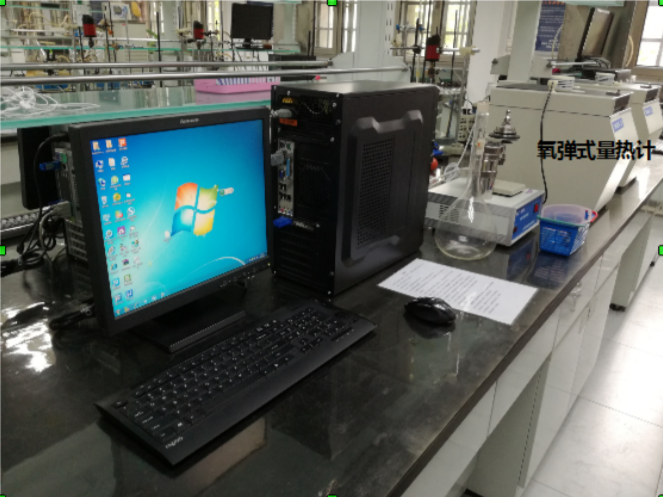
\includegraphics[width=400pt]{Equipment01.pdf}
\end{figure}


本次实验的仪器除上图所示外,还用到分析天平(精度为0.0001g)、压片机。
本次实验用到的两种主要药品如下表所示:
\newpage
\begin{table}[!ht]
\centering
\caption{实验药品一览表}
\begin{tabular}{cccc}
\hline
药品名称 & 英文名称 & 分子量 & 标况下燃烧焓(kJ/mol)\\
\hline
苯甲酸 & benzonic acid & 122 & 3228\\
萘 & naphthalene & 128 & 5156 \\
\hline
\end{tabular}
\end{table}


\subsection{\textbf{\fontsize{12pt}{\baselineskip}{实验条件}}}
本次实验在室温,一个大气压的条件下进行。
\subsection{\textbf{\fontsize{12pt}{\baselineskip}{实验操作步骤及方法要点}}}
\begin{enumerate}
\item 用天平粗称0.8g左右的苯甲酸样品,进行压片,用棉线和镍丝绑好样品,固定在氧弹装置的燃烧杯中。
\item 用万用表检查电路是否接通,若无异常情况则用高压氧气瓶往氧弹装置里充气。
\item 结合计算机上软件的指示,进行水温的调节,使外筒的温度高于内筒约0.8-1\degree C,并控制内筒水量为2L。
\item 用计算机上的软件自动控制点火的时机和温度的采集。
\item 换称0.6g左右的萘样品,重复以上过程,利用苯甲酸作为标定样品,计算出萘的燃烧热。
\end{enumerate}
\section{\textbf{\fontsize{12pt}{\baselineskip}{结果与讨论}}}
\subsection{\textbf{\fontsize{12pt}{\baselineskip}{原始实验数据}}}
燃烧前后称量各反应物的质量如下表所示;
\begin{table}[!ht]
\centering
\caption{反应物质量一览表(单位:g)}
\begin{tabular}{ccccc}
\hline
燃烧物名称 & 燃烧质量& 棉线 & 反应前镍丝 & 反应后镍丝\\
\hline
苯甲酸 & 0.8925 & 0.0139 & 0.0297 & 0.0287\\
萘 & 0.5925 & 0.0146 & 0.0283 & 0.0240 \\
\hline
\end{tabular}
\end{table}
苯甲酸燃烧过程温度-时间变化曲线如下图所示:

\begin{figure}[!ht]
  \centering
  \subfloat[][苯甲酸燃烧过程温度-时间变化曲线]{
  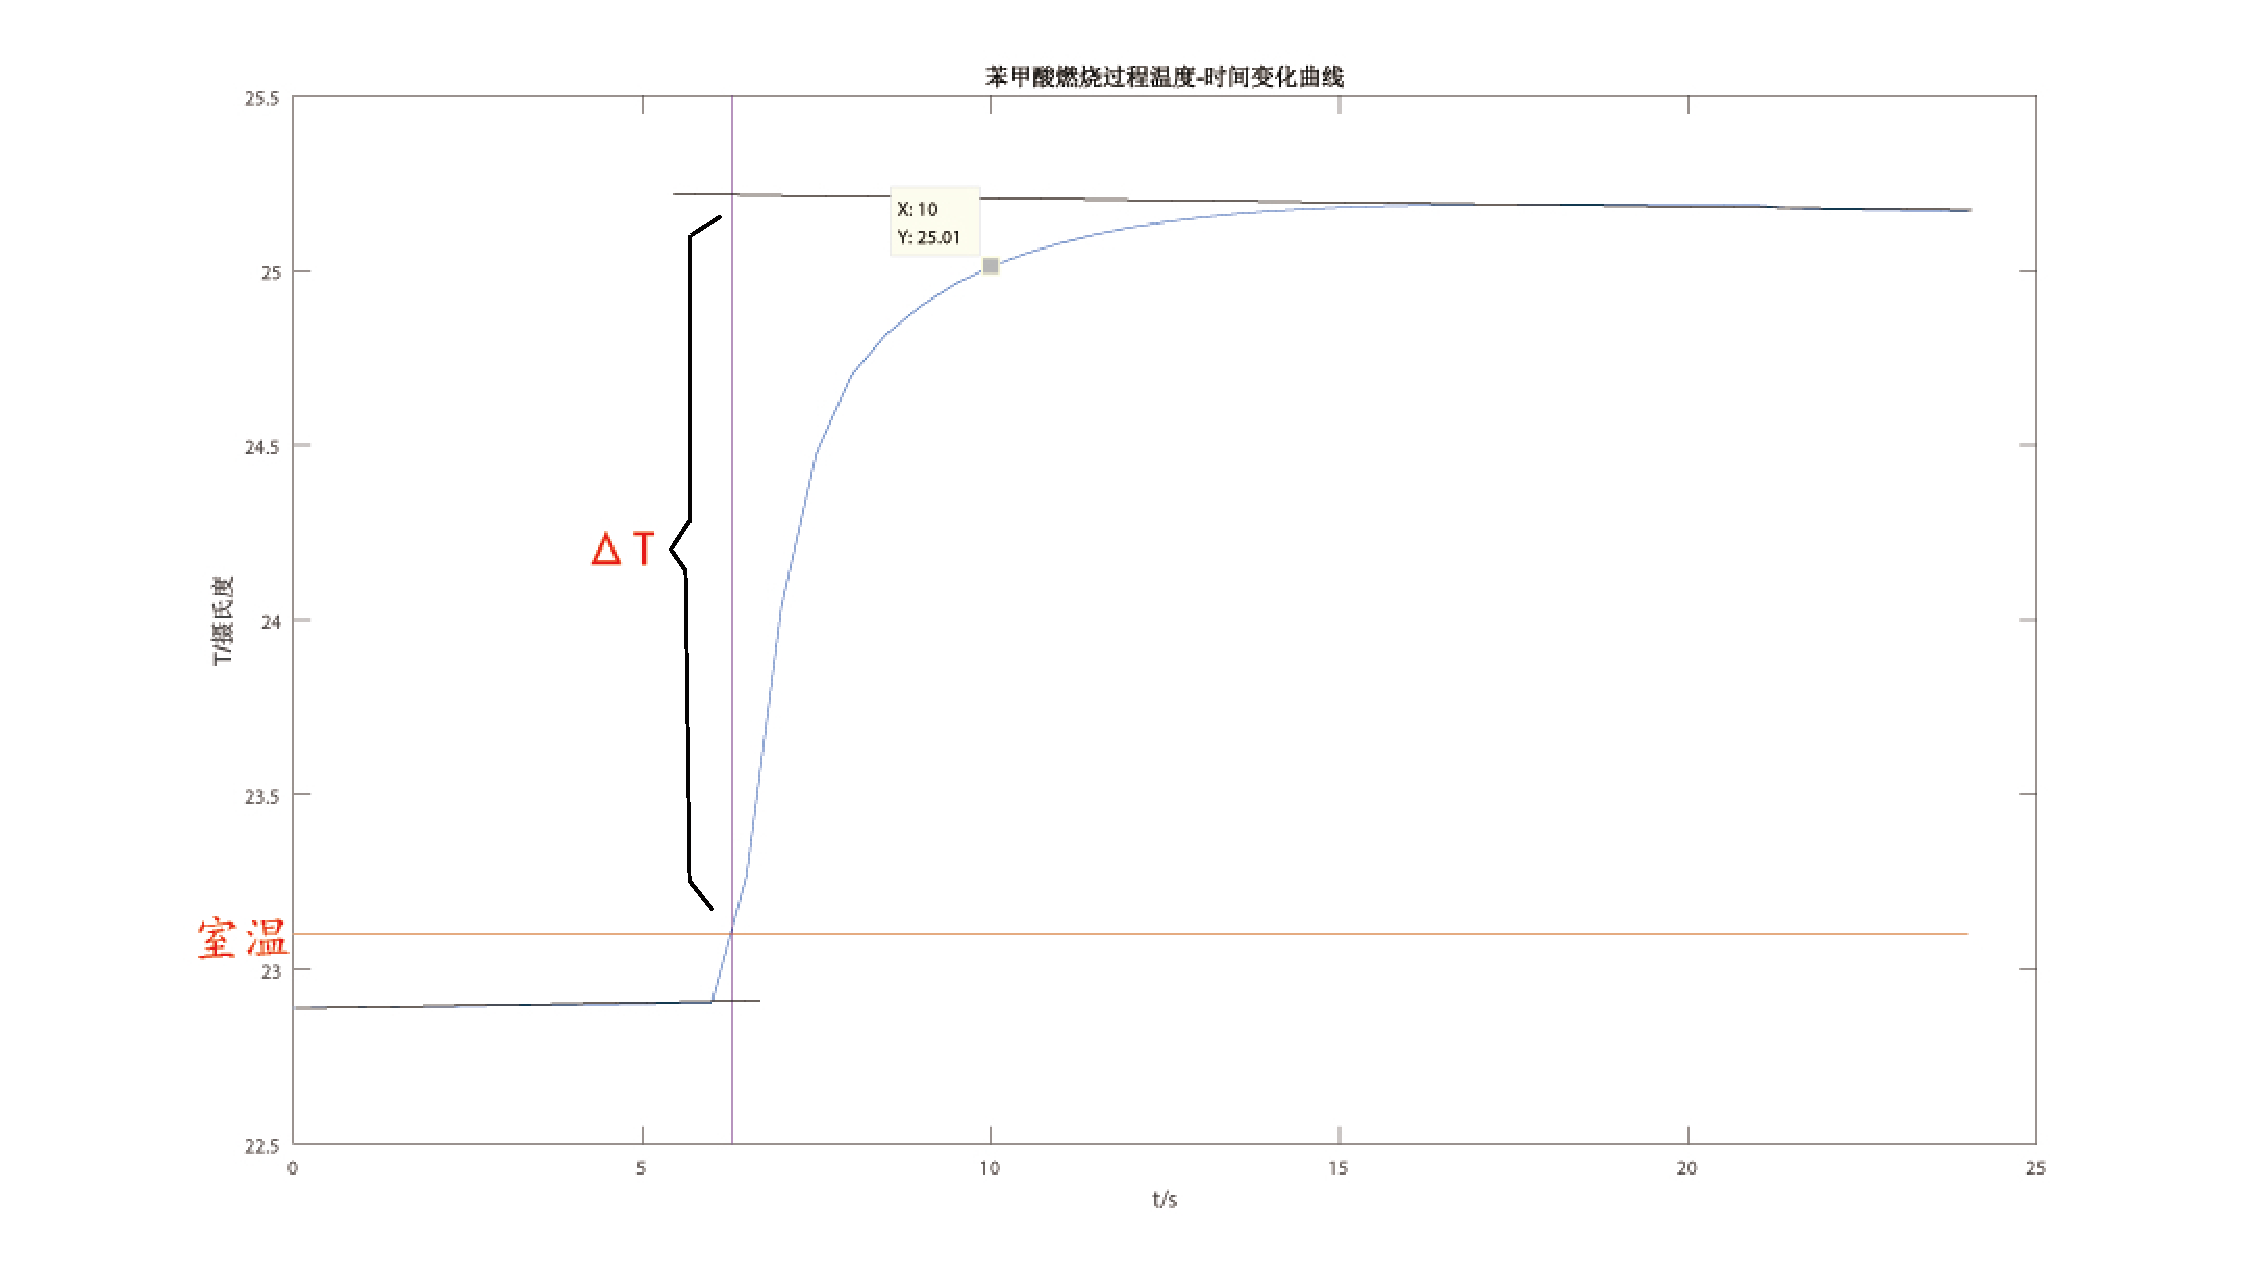
\includegraphics[height=6cm]{image/figure1.pdf}}
  \subfloat[][萘燃烧过程温度-时间变化曲线]{
  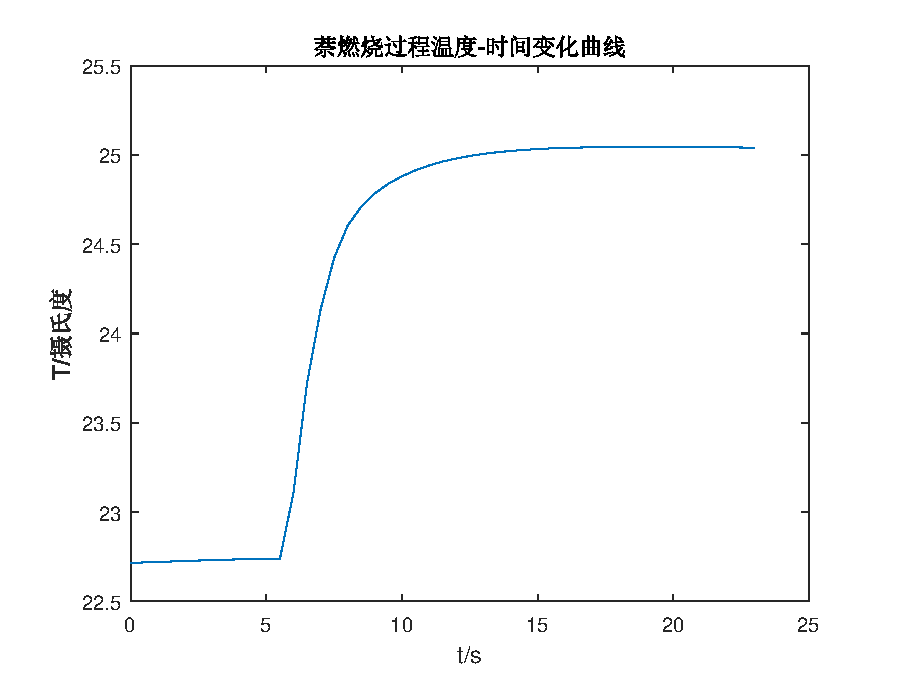
\includegraphics[height=6cm]{image/figure2.eps}}
\end{figure}

\subsection{\textbf{\fontsize{12pt}{\baselineskip}{计算的数据、结果}}}


由公式
\begin{equation}
-\frac{m}{M_r}Q_v-Q_{igniter}l_{igniter}=W\Delta T
\end{equation}
及表格中的数据实际计算发现点火丝和棉线由于质量很少,所产生的热量与有机物相比可以忽略,于是可推出萘的恒压
燃烧热的计算公式为:
\begin{equation}
\frac{Q_b m_b}{\Delta T_b M_b}=\frac{Q_n m_n}{\Delta T_n M_n}
\end{equation}
其中下标b和n分别表示苯甲酸和萘的相关参量。
由恒压燃烧热$Q_V$进一步可计算出燃烧焓,公式为:
\begin{equation}
\Delta H=Q_V+\Delta n R T
\end{equation}
其中$\Delta n$无单位,数值上等于该有机物样品完全燃烧前后气体体积的变化。上式虽在标况(0\degree C)下,但计算发现 $\Delta n RT$相比$Q_V$为小量,可以忽略。于是得到两物种燃烧焓的近似公式:
\begin{equation}
\frac{{\Delta H}_b m_b}{\Delta T_b M_b}=\frac{{\Delta H}_n m_n}{\Delta T_n M_n}
\end{equation}
计算反应前后温度变化时,记温度突变前的温度为$t_s$,反应后达到的最高温度为$t_e$,$Delta T=t_e-t_s$.
得出苯甲酸燃烧前后内筒水温上升2.287\degree C,萘燃烧前后内筒水温上升2.306\degree C,二者非常接近,因此可近似认为
两种情况下温度变化相等,于是由式(4)可知两种物质燃烧焓之比等于物质的量之比和称量质量比,代入表格中数据计算得
${\Delta H}_n \approx 5102 kJ/mol $

\subsection{\textbf{\fontsize{12pt}{\baselineskip}{讨论分析}}}
本次实验虽然最终结果与温度变化值$\Delta T$关系不大,但这主要是由两次称量质量的比值恰好在$0.9/0.6$的范围内决定的,
做实验时发现燃烧进行得非常快,但水温上升需要一段时间,燃烧后氧弹内壁有生成的液体水附着在上面(燃烧前氧弹内部是干燥
的),下个实验前应先清理。

\section{\textbf{\fontsize{12pt}{\baselineskip}{结论}}}

通过本次实验,我们得出如下结论:
\begin{enumerate}
\item 本次实验使用氧弹式量热计,使有机物的燃烧反应在恒压条件下进行,可以定量测定物质的恒压燃烧热,并进一步推算出
燃烧焓。
\item 由于本次实验测温模块误差比较大,而两次温度比又对物质燃烧热的测定有着非常大的影响,所以通过本实验只能粗测物质
的燃烧热,相对误差可控制在1.5\%的范围内。
\end{enumerate}

\section{\textbf{\fontsize{12pt}{\baselineskip}{参考文献}}}
\begin{thebibliography}{}
\bibitem{Bib1}物理化学实验 \quad 化学工业出版社
\end{thebibliography}
\end{document}